\documentclass{article}

\usepackage[tmargin=2cm,rmargin=1in,lmargin=1in,margin=1in,bmargin=2cm,footskip=.2in]{geometry}
\usepackage[font=small,labelfont=bf]{caption}
\usepackage{graphicx}
\usepackage{listings}
\usepackage{multirow}
\usepackage{color}
\usepackage[T1]{fontenc}
\usepackage{setspace}
\usepackage[ngerman]{babel}
\usepackage{tabularx}
\usepackage[nohyphen]{underscore}

\definecolor{codecomment}{rgb}{0,0.6,0}
\definecolor{codelinenumber}{rgb}{0.5,0.5,0.5}
\definecolor{codestring}{rgb}{0.58,0,0.82}
\definecolor{codebg}{rgb}{0.95, 0.95, 0.95}

\makeatletter
\def\@maketitle{
  \null
  \vskip 4cm
  \begin{center}%
    {%
      \doublespacing
      \Large\bfseries \@title \par
    }
    \vskip 4em
    {\normalsize
      \lineskip .5em
      \begin{tabular}[t]{c}
        \@author
    \end{tabular}\par}
    \vskip 4em
    {\normalsize \textbf{\@date}}
    \vskip 1cm
    \url{https://github.com/bzundel/weather-flosscast}
  \end{center}%
  \par
  \vskip 1.5em}
\makeatother

% Attribution to David Carlisle (@david-carlisle) on TeX StackExchange
% https://tex.stackexchange.com/questions/618849/how-to-create-subsubsubsection
\makeatletter
\renewcommand\paragraph{\@startsection{paragraph}{4}{\z@}%
                                     {-3.25ex\@plus -1ex \@minus -.2ex}%
                                     {1.5ex \@plus .2ex}%
                                     {\normalfont\normalsize\bfseries}}
\setcounter{secnumdepth}{4}
\makeatother

\lstset{
  backgroundcolor=\color{codebg},
  basicstyle=\ttfamily\footnotesize,
  breakatwhitespace=true,
  breaklines=true,
  captionpos=b,
  commentstyle=\color{codecomment},
  escapeinside={\%*}{*)},
  extendedchars=true,
  frame=lines,
  keepspaces=true,
  keywordstyle=\color{blue},
  numbers=left,
  numbersep=10pt,
  numberstyle=\tiny\color{codelinenumber},
  rulecolor=\color{black},
  showspaces=false,
  showstringspaces=false,
  showtabs=false,
  stepnumber=1,
  stringstyle=\color{codestring},
  tabsize=4,
  captionpos=top
}


\usepackage{listings}
\usepackage{hyperref}

\graphicspath{{assets/}}

\title{Weather App "weatherFLOSScast"\\
  {%
    \onehalfspacing
    \begin{large}
    WP-Seminar "Quelloffene Software in der modernen Informatik" Projekt
    \end{large}\\
    \small Unter Beaufsichtigung von Dr. Chris Zimmermann\\
  }
  \begin{normalsize}
    Frankfurt University of Applied Sciences
  \end{normalsize}
}

\author{
  Brychcy, Patryk \\
  \texttt{patryk.brychcy@stud.fra-uas.de}
  \and
  Filatoff, Michael \\
  \texttt{michael.filatoff@stud.fra-uas.de}
  \and
  Fluegel, Dwipa \\
  \texttt{dwipa.fluegel@stud.fra-uas.de}
  \and
  Gavrilov, Sascha \\
  \texttt{sascha.gavrilov@stud.fra-uas.de}
  \and
  Karaman, Deniz \\
  \texttt{deniz.karaman@stud.fra-uas.de}
  \and
  Lepore, Dominik \\
  \texttt{dominik.lepore@stud.fra-uas.de}
  \and
  Zimmermann, Alwin \\
  \texttt{alwin.zimmermann@stud.fra-uas.de}
  \and
  Zundel, Benedikt \\
  \texttt{benedikt.zundel@stud.fra-uas.de}
}

\date{Friday, 2025-06-20}

\begin{document}

\maketitle

\newpage

\tableofcontents

\newpage

\listoffigures
\lstlistoflistings

\newpage

\section{Projektmanagement mit Scrum \& GitHub Projects \small{(Deniz Karaman)}}
Um unseren Entwicklungsprozess agil zu strukturieren, haben wir Scrum mithilfe von GitHub Projects implementiert. Dabei haben wir uns an klassischen Scrum-Prinzipien orientiert und diese wie üblich an unsere Teamgröße und die Projektanforderungen angepasst. Jede Story wird dabei als Issue angelegt.

Zunächst haben wir in unseren Issues sowohl Labels als auch Milestones definiert, um einen schnellen Überblick zu gewährleisten und einzelne Issues entsprechend ihrer Zuordnung hervorzuheben. Da wir unsere Stories im Team abgestimmt und deren Komplexität berücksichtigt haben, gelten die Definition of Done (DoD) sowie die Bewertung als feststehend.

Folgende Labels haben wir definiert: \textit{backend}, \textit{bug}, \textit{documentation}, \textit{enhancement}, \textit{epic}, \textit{frontend}, \textit{story}, \textit{testing}. Zusätzlich zu unseren Labels benötigen wir unterschiedliche Status, für die wir folgende verwenden: \textit{Todo}, \textit{In} \textit{Progress}, \textit{Needs} \textit{Review}, \textit{Done}, \textit{Canceled}.

Durch die Nutzung von Custom Fields vom Typ Iteration können wir unsere Sprints zeitlich organisieren und in wöchentlichen Zyklen abbilden. Bei der Sprintplanung in unseren Meetings haben wir zudem die Möglichkeit, sowohl die Story Points als auch die Priorität (\textit{Low}, \textit{Medium}, \textit{High}, \textit{Critical}) über Custom Fields abzubilden.

Nach Abschluss jedes Sprints haben wir dienstags abends wöchentlich erst eine Retrospektive und anschließend die Sprint-Planung abgehalten. Da nicht immer alle teilnehmen konnten, haben wir unsere Entwicklung in den User Stories protokolliert, um sie für alle nachvollziehbar zu machen.

\subsection{Darstellung Boards}
\begin{figure}[h]
  \caption{Screenshot der GitHub Projects Ansicht des Backlogs}
  \centering
  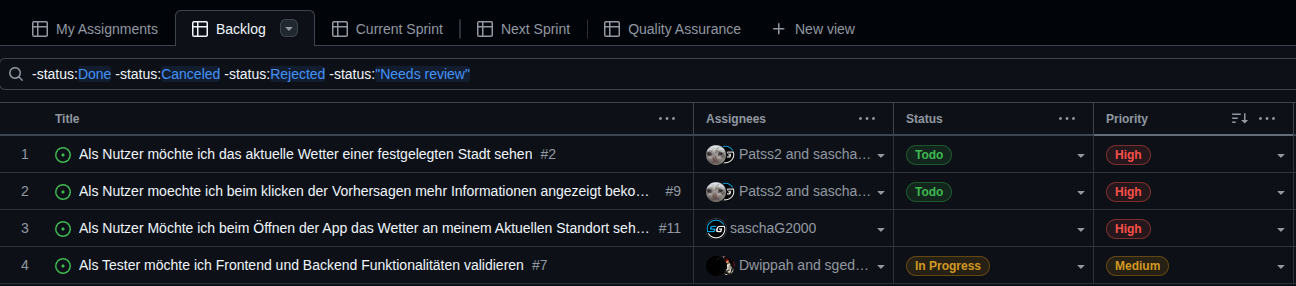
\includegraphics[width=\textwidth]{backlog.png}
\end{figure}

Um die Übersichtlichkeit weiter zu erhöhen, haben wir für jede Board-Ansicht vordefinierte Filter konfiguriert.

So erhält jede Ansicht genau die Issues, die für den jeweiligen Arbeitsschritt relevant sind, und das Team behält jederzeit den passenden Fokus.

\begin{figure}[h]
  \caption{Screenshot der GitHub Projects Ansicht der Quality Assurance}
  \centering
  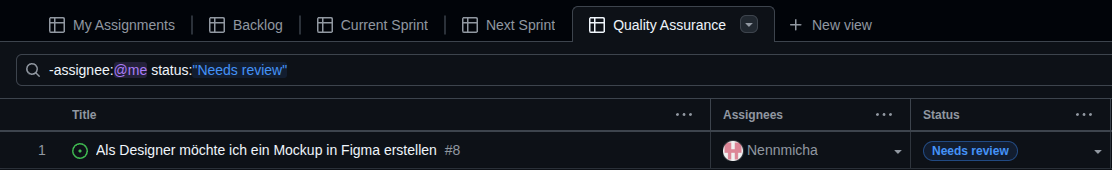
\includegraphics[width=\textwidth]{quality_assurance.png}
\end{figure}

\begin{itemize}
  \item \textbf{Backlog}: Alle geplanten User Stories und Tasks
  \item \textbf{Current Sprint}: Die aktuell bearbeiteten Items
  \item \textbf{Next Sprint}: Vorgemerkte Stories für den nächsten Sprint
  \item \textbf{Quality Assurance}: Abgenommene Features in der Testphase
  \item \textbf{Done}: Abgeschlossene Stories
\end{itemize}

Jeder Eintrag auf dem Board ist als GitHub Issue angelegt und hat folgende Felder
	
\begin{enumerate}
  \item Story Points (zur Aufwandsschätzung in Fibonacci)
  \item Priority-Labels (\textit{Low}, \textit{Medium}, \textit{High}, \textit{Critical})
  \item Sprint-Labels (z. B. \textit{Sprint1}, \textit{Sprint2}, etc.)
  \item Status-Labels (\textit{Todo}, \textit{In Progress}, \textit{Needs review}, \textit{Done}, \textit{Canceled})
\end{enumerate}

\begin{figure}[h]
  \caption{Screenshot der GitHub Ansicht einer Story}
  \centering
  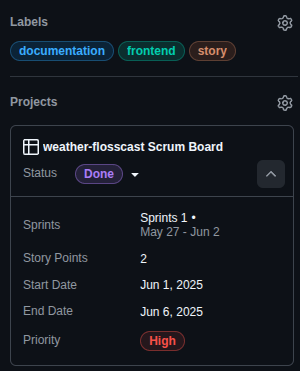
\includegraphics[width=.3\textwidth]{overview.png}
\end{figure}

Durch diese enge Verzahnung von Issue-Tracking, Code-Repositories und agilen Meetings erreichen wir eine hohe Transparenz, schnelle Feedback-Zyklen und eine stetige Verbesserung unseres Workflows.

\section{Product ownership \small{(Alwin Zimmermann)}}
\subsection{Aufgaben des Product Owners}
In der Rolle des Product Owners war es erforderlich, eine präzise Definition des Projekts zu formulieren. Von entscheidender Bedeutung war die Erstellung von Anforderungen sowie die Ausarbeitung der verschiedenen User-Stories . Das Produkt muss den Erwartungen der Stakeholder entsprechen. Die Pflege des Backlogs zählt ebenfalls zu den Aufgaben des Product Owners, um den Fortschritt des Projekts zu dokumentieren.

\subsection{Probleme}
Eine der größten Herausforderungen im Team bestand in der Organisation regelmäßiger Besprechungen. Obwohl unsere Stundenpläne und täglichen Abläufe variieren, haben wir es geschafft, uns in regelmäßigen Abständen zuverlässig zu treffen. Der Austausch mit dem Scrum Master erwies sich als äußerst nützlich, ebenso wie die Kooperation innerhalb des gesamten Entwicklerteams.

\subsection{Ziel der Entwiklung}
Das Ziel des Projekts bestand darin, eine Wetteranwendung für das Android-Betriebssystem zu entwickeln. Die Anforderungen bestanden darin, dass die Anwendung bestimmte Vorgaben erfüllt und den Erwartungen der Stakeholder gerecht wird.
Im Folgenden werde ich auf die von uns erstellten Reqirements eingehen und die daraus resultierenden User-Stories erläutern.

\subsection{Requirements}
In diesem Teil gehe ich auf die Requirements ein. Diese beziehen sich auf die unten stehenden User-Stories. Die Kern-Requirements dienen als erste Anhaltspunkte, was der Product Owner verlangt und welche Kernfunktionalitäten wichtig sind.

\subsection{Kernfunktionen (Hohe Priorität) \small{(Alwin Zimmermann)}}

\subsubsection{Automatisches Anzeigen des aktuellen Wetters am Standort (US-001)}
\begin{itemize}
    \item Beim Start der App wird das aktuelle Wetter für den geografischen Standort des Nutzers automatisch und ohne manuelle Interaktion angezeigt.
    \item Ziel ist es, dem Nutzer sofortige und präzise Informationen über seine unmittelbare Umgebung zu liefern.
\end{itemize}

\subsubsection{Städtesuche und -verwaltung (US-002, US-005)}
\begin{itemize}
    \item Nutzer müssen in der Lage sein, Städte zu suchen (z.B. über eine Suchleiste).
    \item Gefundene Städte können einer personalisierten Favoritenliste hinzugefügt werden.
    \item Das Wetter der in der Liste gespeicherten Städte muss abrufbar sein.
    \item Nutzer müssen die Möglichkeit haben, Städte aus ihrer Favoritenliste zu entfernen, um die Ansicht zu optimieren.
\end{itemize}

\subsubsection{Wettervorhersage für zukünftige Tage (US-003, US-004)}
\begin{itemize}
    \item Die App muss eine Wettervorhersage für die kommenden Tage am aktuellen Standort des Nutzers anzeigen können.
    \item Die App muss eine Wettervorhersage für die kommenden Tage der in der Favoritenliste gespeicherten Städte anzeigen können.
    \item Ziel ist es, den Nutzer umfassend über zukünftige Wettersituationen zu informieren.
\end{itemize}

\subsection{Offline-Funktionalität (Mittlere Priorität)}

\subsubsection{Offline-Zugriff auf das letzte Wetter am Standort (US-005)}
\begin{itemize}
    \item Wenn keine Internetverbindung besteht, soll die App die zuletzt abgerufenen Wetterdaten für den aktuellen Standort anzeigen.
    \item Diese Funktion stellt sicher, dass der Nutzer auch ohne Internetverbindung grundlegende Informationen erhält.
\end{itemize}

\subsubsection{Offline-Zugriff auf das Wetter gespeicherter Städte (US-006)}
\begin{itemize}
    \item Die App muss die zuletzt abgerufenen Wetterdaten für die in der Favoritenliste gespeicherten Städte auch im Offline-Modus anzeigen können.
    \item Die angezeigten Offline-Daten sollten nicht älter als das Ende des letzten verfügbaren Forecasts sein, um eine gewisse Relevanz zu gewährleisten.
\end{itemize}

\subsubsection{Fehlermeldung bei fehlender Internetverbindung (US-007)}
\begin{itemize}
    \item Bei fehlender oder unterbrochener Internetverbindung muss eine eindeutige Fehlermeldung angezeigt werden, die den Nutzer über den Offline-Status informiert.
\end{itemize}

\subsection{App-Informationen und Hilfe (Niedrige Priorität)}

\subsubsection{Hilfefunktion und Impressum (US-008)}
\begin{itemize}
    \item Die App soll eine Hilfefunktion bereitstellen, die dem Nutzer die Bedienung der App erklärt.
    \item Dieser Bereich muss auch ein Impressum enthalten, das Informationen über den Entwickler und die Lizenz der App bereitstellt.
\end{itemize}

\subsection{User-Stories}
In diesem teil sammele und beschreibe ich die User Stories für das Projekt \textbf{Weather-flosscast}. Jede User Story repräsentiert eine Anforderung aus der Perspektive eines Benutzers und dient als Grundlage für die Entwicklung und Schätzung.

\subsubsection{Übersicht der User Stories}
Um eine klare Übersicht zu gewährleisten, sind die wichtigsten Metadaten der User Stories in der folgenden Tabelle zusammengefasst. Detaillierte Beschreibungen und Akzeptanzkriterien finden sich in den nachfolgenden Abschnitten.

\setlength{\LTpre}{0pt} % Kein zusätzlicher Platz vor der longtable
\setlength{\LTpost}{0pt} % Kein zusätzlicher Platz nach der longtable

%\small % Makes the text in the table slightly smaller
%\begin{longtable}{|>{\RaggedRight}X|c|c|}
%\hline
%\textbf{Beschreibung} & \textbf{US} & \textbf{Priorität} \\
%\hline
%\endhead % End of the table header (repeated on each page)
%
%\hline
%\multicolumn{3}{|r|}{Fortsetzung auf nächster Seite} \\
%\hline
%\endfoot % Footer for page breaks
%
%\hline
%\endlastfoot % Footer for the end of the table
%
%Als Nutzer möchte ich beim Öffnen der App das aktuelle Wetter für meinen Standort sehen. & US-001 & Hoch \\
%Als Nutzer möchte ich nach Städten suchen und sie einer Liste hinzufügen können. & US-002 & Hoch \\
%Als Nutzer möchte ich das Wetter der zukünftigen Tage an meinem Standort sehen. & US-003 & Hoch \\
%Als Nutzer möchte ich das zukünftige Wetter von gespeicherten Städten sehen. & US-004 & Hoch \\
%Als Nutzer möchte ich Städte aus meiner Liste löschen können. & US-005 & Hoch \\
%Als Nutzer möchte ich auch ohne Internet das letzte aktuelle Wetter an meinem Standort sehen. & US-006 & Mittel \\
%Als Nutzer möchte ich auch ohne Internet das Wetter aus zuvor hinzugefügten Städten sehen. & US-007 & Mittel \\
%Als Nutzer möchte ich eine Fehlermeldung sehen, wenn ich kein Internet habe. & US-008 & Mittel \\
%Als Nutzer möchte ich eine Hilfefunktion und ein Impressum in der App finden. & US-009 & Niedrig \\
%\end{longtable}

\normalsize
\subsection{Detaillierte User Story Beschreibungen}

In diesem Abschnitt werden die einzelnen User Stories ausführlich beschrieben, inklusive ihrer Akzeptanzkriterien.
\newpage
\subsubsection{User Story: Als Nutzer möchte ich beim Öffnen der App das aktuelle Wetter für meinen Standort sehen.}
\textcolor{storyblue}{\textbf{ID:}} US-001 \\
\textcolor{storyblue}{\textbf{Priorität:}} Hoch \\
\textcolor{storyblue}{\textbf{Status:}} Neu \\
\textcolor{storyblue}{\textbf{Verantwortlicher:}} Siehe GitHub \\
\textcolor{storyblue}{\textbf{Geschätzte Story Points:}} 8

\vspace{0.5em}

\textcolor{storygreen}{\textbf{Als}} \textit{Nutzer} \\
\textcolor{storygreen}{\textbf{möchte ich}} \textit{die App öffnen und ohne mein Zutun das aktuelle Wetter für meinen Standort angezeigt bekommen}, \\
\textcolor{storygreen}{\textbf{damit}} \textit{ich genaue Infos über meinen Standort habe}.

\vspace{1em}

\paragraph{Details und Beschreibung}
Diese User Story beschreibt die Kernfunktionalität der App, bei der der Nutzer sofort nach dem Start die relevantesten Wetterdaten für seinen aktuellen geografischen Standort sieht. Dies erfordert Zugriff auf die Standortdienste des Geräts und die Abfrage einer Wetter-API.

\vspace{0.5em}
\hrule

\paragraph{Akzeptanzkriterien}
\begin{itemize}
    \item Die App startet erfolgreich und fordert ggf. die Standortberechtigung an.
    \item Nach Erteilung der Berechtigung wird das aktuelle Wetter (Temperatur, Wetterlage, ggf. Wind, Luftfeuchtigkeit) für den aktuellen Standort angezeigt.
    \item Bei fehlender Standortberechtigung wird eine informative Meldung angezeigt und die Möglichkeit geboten, die Berechtigung zu aktivieren oder manuell eine Stadt einzugeben (siehe US-002).
    \item Die angezeigten Daten sind aktuell und stammen von einer zuverlässigen Wetter-API.
\end{itemize}

\vspace{0.5em}
\hrule

\paragraph{Abhängigkeiten}
* Benötigt eine Wetter-API-Integration.
* Benötigt Zugriff auf Standortdienste des Geräts.

\paragraph{Anmerkungen/Diskussion}
* 05.06.2025: Klärung, welche spezifischen Wetterdaten (z.B. Regenwahrscheinlichkeit, UV-Index) standardmäßig angezeigt werden sollen.

\clearpage

\subsubsection{User Story: Als Nutzer möchte ich nach Städten suchen und sie einer Liste hinzufügen können.}
\textcolor{storyblue}{\textbf{ID:}} US-002 \\
\textcolor{storyblue}{\textbf{Priorität:}} Hoch \\
\textcolor{storyblue}{\textbf{Status:}} Neu \\
\textcolor{storyblue}{\textbf{Verantwortlicher:}} Sihe GitHub \\
\textcolor{storyblue}{\textbf{Geschätzte Story Points:}} 6

\vspace{0.5em}

\textcolor{storygreen}{\textbf{Als}} \textit{Nutzer} \\
\textcolor{storygreen}{\textbf{möchte ich}} \textit{nach Städten suchen und sie einer Liste hinzufügen können}, \\
\textcolor{storygreen}{\textbf{damit}} \textit{ich nachher auch das Wetter in diesen Städten anschauen kann}.

\vspace{1em}

\paragraph{Details und Beschreibung}
Diese User Story ermöglicht es dem Nutzer, Städte manuell hinzuzufügen, um deren Wetter zu verfolgen. Dies beinhaltet eine Suchfunktion und die Möglichkeit, ausgewählte Städte in einer persistenten Liste zu speichern.

\vspace{0.5em}
\hrule

\paragraph{Akzeptanzkriterien}
\begin{itemize}
    \item Es gibt ein Suchfeld, über das der Nutzer Städte eingeben kann.
    \item Die Suchergebnisse zeigen relevante Städte basierend auf der Eingabe an (z.B. mit Autovervollständigung).
    \item Der Nutzer kann eine Stadt aus den Suchergebnissen auswählen und diese zu einer Liste hinzufügen.
    \item Die hinzugefügten Städte bleiben auch nach dem Schließen der App in der Liste gespeichert.
    \item Die Liste der Städte ist übersichtlich dargestellt und leicht zugänglich.
\end{itemize}

\vspace{0.5em}
\hrule

\paragraph{Abhängigkeiten}
* Benötigt eine Stadt-Geocoding-API oder ähnliche Datenbank.
* Benötigt eine persistente Speicherung der Städte.

\paragraph{Anmerkungen/Diskussion}
* 05.06.2025: Überlegen, ob es eine Begrenzung für die Anzahl der speicherbaren Städte geben soll.

\clearpage

\subsubsection{User Story: Als Nutzer möchte ich das Wetter der zukünftigen Tage an meinem Standort sehen.}
\textcolor{storyblue}{\textbf{ID:}} US-003 \\
\textcolor{storyblue}{\textbf{Priorität:}} Hoch \\
\textcolor{storyblue}{\textbf{Status:}} Neu \\
\textcolor{storyblue}{\textbf{Verantwortlicher:}} Siehe GitHub \\
\textcolor{storyblue}{\textbf{Geschätzte Story Points:}} 8

\vspace{0.5em}

\textcolor{storygreen}{\textbf{Als}} \textit{Nutzer} \\
\textcolor{storygreen}{\textbf{möchte ich}} \textit{das Wetter der zukünftigen Tage an meinem Standort sehen}, \\
\textcolor{storygreen}{\textbf{damit}} \textit{ich genau über die Wettersituation informiert bin}.

\vspace{1em}

\paragraph{Details und Beschreibung}
Diese User Story erweitert die Standortanzeige um eine Vorhersage für die kommenden Tage (z.B. 3-5 Tage). Der Nutzer soll auf einen Blick sehen können, wie sich das Wetter entwickelt.

\vspace{0.5em}
\hrule

\paragraph{Akzeptanzkriterien}
\begin{itemize}
    \item Neben dem aktuellen Wetter werden Vorhersagen für die nächsten 3/5 Tage für den aktuellen Standort angezeigt.
    \item Jede Tagesvorhersage zeigt mindestens die Höchst- und Tiefsttemperatur und die Wetterlage an (z.B. Sonnensymbol, Regensymbol).
    \item Die Vorhersage ist klar und übersichtlich dargestellt.
    \item Die Daten stammen von der integrierten Wetter-API.
\end{itemize}

\vspace{0.5em}
\hrule

\paragraph{Abhängigkeiten}
* Benötigt eine Wetter-API, die Vorhersagedaten bereitstellt.
* Abhängig von US-001 (Standortbestimmung).

\paragraph{Anmerkungen/Diskussion}
* 05.06.2025: Festlegen, wie viele Tage die Vorhersage umfassen soll (z.B. 3 oder 5 Tage).

\clearpage

\subsubsection{User Story: Als Nutzer möchte ich das zukünftige Wetter von gespeicherten Städten sehen.}
\textcolor{storyblue}{\textbf{ID:}} US-004 \\
\textcolor{storyblue}{\textbf{Priorität:}} Hoch \\
\textcolor{storyblue}{\textbf{Status:}} Neu \\
\textcolor{storyblue}{\textbf{Verantwortlicher:}} Siehe GitHub \\
\textcolor{storyblue}{\textbf{Geschätzte Story Points:}} 8

\vspace{0.5em}

\textcolor{storygreen}{\textbf{Als}} \textit{Nutzer} \\
\textcolor{storygreen}{\textbf{möchte ich}} \textit{das zukünftige Wetter einer der zuvor festgelegten Städte sehen}, \\
\textcolor{storygreen}{\textbf{damit}} \textit{ich über die Situation an einem anderen Ort Bescheid weiß}.

\vspace{1em}

\paragraph{Details und Beschreibung}
Diese User Story ermöglicht es dem Nutzer, die Wettervorhersage für die Städte einzusehen, die er zu seiner Liste hinzugefügt hat.

\vspace{0.5em}
\hrule

\paragraph{Akzeptanzkriterien}
\begin{itemize}
    \item Der Nutzer kann eine gespeicherte Stadt aus der Liste auswählen.
    \item Nach Auswahl der Stadt werden die aktuellen Wetterdaten und die Vorhersage für die nächsten [X] Tage für diese Stadt angezeigt.
    \item Die Anzeige der Vorhersage ist konsistent mit der Anzeige für den eigenen Standort (US-003).
\end{itemize}

\vspace{0.5em}
\hrule

\paragraph{Abhängigkeiten}
* Abhängig von US-002 (Städte hinzufügen und speichern).
* Benötigt Wetter-API für Vorhersagedaten für beliebige Orte.

\paragraph{Anmerkungen/Diskussion}
* 05.06.2025: Wie wird zwischen den Städten gewechselt? (z.B. Swipe-Gesten, Dropdown-Menü).

\clearpage

\subsubsection{User Story: Als Nutzer möchte ich Städte aus meiner Liste löschen können.}
\textcolor{storyblue}{\textbf{ID:}} US-005 \\
\textcolor{storyblue}{\textbf{Priorität:}} Hoch \\
\textcolor{storyblue}{\textbf{Status:}} Neu \\
\textcolor{storyblue}{\textbf{Verantwortlicher:}} Siehe gitHub \\
\textcolor{storyblue}{\textbf{Geschätzte Story Points:}} 3

\vspace{0.5em}

\textcolor{storygreen}{\textbf{Als}} \textit{Nutzer} \\
\textcolor{storygreen}{\textbf{möchte ich}} \textit{Städte aus der Liste löschen können}, \\
\textcolor{storygreen}{\textbf{damit}} \textit{ich meine Ansicht verbessern und vereinfachen kann}.

\vspace{1em}

\paragraph{Details und Beschreibung}
Diese User Story bietet die Möglichkeit, nicht mehr benötigte Städte aus der Favoritenliste des Nutzers zu entfernen.

\vspace{0.5em}
\hrule

\paragraph{Akzeptanzkriterien}
\begin{itemize}
    \item Der Nutzer kann eine Option zum Löschen von Städten in der Liste finden (z.B. Bearbeiten-Button, Swipe-Geste).
    \item Nach Bestätigung wird die Stadt aus der Liste entfernt.
    \item Die Änderungen werden dauerhaft gespeichert.
    \item Der Nutzer erhält eine visuelle Rückmeldung über das Löschen der Stadt.
\end{itemize}

\vspace{0.5em}
\hrule

\paragraph{Abhängigkeiten}
* Abhängig von US-002 (Städte hinzufügen und speichern).

\paragraph{Anmerkungen/Diskussion}
* 05.06.2025: Bestätigungsdialog für das Löschen einer Stadt implementieren, um versehentliches Löschen zu verhindern.

\clearpage

\subsubsection{User Story: Als Nutzer möchte ich auch ohne Internet das letzte aktuelle Wetter an meinem Standort sehen.}
\textcolor{storyblue}{\textbf{ID:}} US-006 \\
\textcolor{storyblue}{\textbf{Priorität:}} Mittel \\
\textcolor{storyblue}{\textbf{Status:}} Neu \\
\textcolor{storyblue}{\textbf{Verantwortlicher:}} Siehe GitHub \\
\textcolor{storyblue}{\textbf{Geschätzte Story Points:}} 5

\vspace{0.5em}

\textcolor{storygreen}{\textbf{Als}} \textit{Nutzer} \\
\textcolor{storygreen}{\textbf{möchte ich}} \textit{auch ohne Internet das letzte aktuelle Wetter an meinem Standort sehen}, \\
\textcolor{storygreen}{\textbf{damit}} \textit{ich auch ohne Internet die letzten zuverlässigen Wetterzustände sehen kann}.

\vspace{1em}

\paragraph{Details und Beschreibung}
Diese User Story beschreibt die Offline-Fähigkeit der App für den aktuellen Standort. Die zuletzt geladenen Wetterdaten sollen gespeichert und bei fehlender Internetverbindung angezeigt werden.

\vspace{0.5em}
\hrule

\paragraph{Akzeptanzkriterien}
\begin{itemize}
    \item Bei bestehender Internetverbindung werden die Wetterdaten des Standorts lokal gespeichert.
    \item Wenn die Internetverbindung unterbrochen ist, werden die zuletzt gespeicherten Wetterdaten für den aktuellen Standort angezeigt.
    \item Es wird ein Hinweis angezeigt, dass die Daten nicht aktuell sind und wann sie zuletzt aktualisiert wurden.
    \item Der Wert sollte nicht älter als das Ende des Forecasts sein. (Die Daten sollten innerhalb des Gültigkeitszeitraums der letzten Vorhersage liegen).
\end{itemize}

\vspace{0.5em}
\hrule

\paragraph{Abhängigkeiten}
* Abhängig von US-001 (Aktuelles Wetter am Standort).
* Benötigt lokale Speichermechanismen.

\paragraph{Anmerkungen/Diskussion}
* 05.06.2025: Festlegen, wie lange die gecachten Daten als "zuverlässig" gelten (z.B. maximal 1-2 Stunden für aktuelle Daten, bis zum Ende des Forecasts für Vorhersagen).

\clearpage

\subsubsection{User Story: Als Nutzer möchte ich auch das Wetter aus zuvor hinzugefügten Städten sehen ohne Internet zu haben.}
\textcolor{storyblue}{\textbf{ID:}} US-007 \\
\textcolor{storyblue}{\textbf{Priorität:}} Mittel \\
\textcolor{storyblue}{\textbf{Status:}} Neu \\
\textcolor{storyblue}{\textbf{Verantwortlicher:}} Siehe GitHub \\
\textcolor{storyblue}{\textbf{Geschätzte Story Points:}} 5

\vspace{0.5em}

\textcolor{storygreen}{\textbf{Als}} \textit{Nutzer} \\
\textcolor{storygreen}{\textbf{möchte ich}} \textit{auch das Wetter aus zuvor hinzugefügten Städten sehen, ohne Internet zu haben}. \\
\textcolor{storygreen}{\textbf{Der Wert sollte nicht älter als das Ende des Forecasts sein.}}

\vspace{1em}

\paragraph{Details und Beschreibung}
Diese User Story erweitert die Offline-Funktionalität auf die vom Nutzer gespeicherten Städte. Die zuletzt abgerufenen Wetterdaten und Vorhersagen für diese Städte sollen ebenfalls gecacht und bei fehlender Internetverbindung angezeigt werden.

\vspace{0.5em}
\hrule

\paragraph{Akzeptanzkriterien}
\begin{itemize}
    \item Bei bestehender Internetverbindung werden die Wetterdaten der gespeicherten Städte lokal gespeichert.
    \item Wenn die Internetverbindung unterbrochen ist, werden die zuletzt gespeicherten Wetterdaten und Vorhersagen für die hinzugefügten Städte angezeigt.
    \item Es wird ein Hinweis angezeigt, dass die Daten nicht aktuell sind und wann sie zuletzt aktualisiert wurden.
    \item Die angezeigten Wetterdaten und Vorhersagen sollten nicht älter sein als das Ende des letzten abgerufenen Forecasts.
\end{itemize}

\vspace{0.5em}
\hrule

\paragraph{Abhängigkeiten}
* Abhängig von US-002 (Städte hinzufügen), US-004 (Zukünftiges Wetter gespeicherter Städte).
* Benötigt lokale Speichermechanismen.

\paragraph{Anmerkungen/Diskussion}
* 05.06.2025: Speicherkapazität der App für Offline-Daten berücksichtigen, insbesondere bei vielen gespeicherten Städten.

\clearpage

\subsubsection{User Story: Als Nutzer möchte ich eine Fehlermeldung sehen, wenn ich kein Internet habe.}
\textcolor{storyblue}{\textbf{ID:}} US-008 \\
\textcolor{storyblue}{\textbf{Priorität:}} Mittel \\
\textcolor{storyblue}{\textbf{Status:}} Neu \\
\textcolor{storyblue}{\textbf{Verantwortlicher:}} Siehe GitHub \\
\textcolor{storyblue}{\textbf{Geschätzte Story Points:}} 1

\vspace{0.5em}

\textcolor{storygreen}{\textbf{Als}} \textit{Nutzer} \\
\textcolor{storygreen}{\textbf{möchte ich}} \textit{dass es eine Fehlermeldung gibt}, \\
\textcolor{storygreen}{\textbf{damit}} \textit{ich weiß, dass ich aktuell kein Internet habe}.

\vspace{1em}

\paragraph{Details und Beschreibung}
Diese User Story stellt sicher, dass der Nutzer klar über den Verbindungsstatus der App informiert wird, insbesondere wenn keine Internetverbindung verfügbar ist und daher keine aktuellen Wetterdaten abgerufen werden können.

\vspace{0.5em}
\hrule

\paragraph{Akzeptanzkriterien}
\begin{itemize}
    \item Wenn die App versucht, Wetterdaten abzurufen und keine Internetverbindung besteht, wird eine sichtbare Fehlermeldung angezeigt (z.B. ein Banner oder Toast-Nachricht).
    \item Die Fehlermeldung informiert den Nutzer klar darüber, dass keine Verbindung besteht.
    \item Die Fehlermeldung verschwindet automatisch, sobald die Verbindung wiederhergestellt ist, oder bietet die Möglichkeit, sie manuell zu schließen.
    \item Die Fehlermeldung sollte die primäre Anzeige nicht überdecken.
\end{itemize}

\vspace{0.5em}
\hrule

\paragraph{Abhängigkeiten}
* Benötigt eine Netzwerkstatusprüfung.

\paragraph{Anmerkungen/Diskussion}
* 05.06.2025: Formulierung der Fehlermeldung abstimmen. Soll sie auch auf die Offline-Funktionalität hinweisen?

\clearpage

\subsubsection{User Story: Als Nutzer möchte ich eine Hilfefunktion und ein Impressum in der App finden.}
\textcolor{storyblue}{\textbf{ID:}} US-009 \\
\textcolor{storyblue}{\textbf{Priorität:}} Niedrig \\
\textcolor{storyblue}{\textbf{Status:}} Neu \\
\textcolor{storyblue}{\textbf{Verantwortlicher:}} Siehe GitHub \\
\textcolor{storyblue}{\textbf{Geschätzte Story Points:}} 2

\vspace{0.5em}

\textcolor{storygreen}{\textbf{Als}} \textit{Nutzer} \\
\textcolor{storygreen}{\textbf{möchte ich}} \textit{eine Hilfefunktion anklicken können}, \\
\textcolor{storygreen}{\textbf{damit}} \textit{ich die App erklärt bekomme und sehen kann, von wem sie kommt und mit welcher Lizenz sie ist (Impressum und Hilfe)}.

\vspace{1em}

\paragraph{Details und Beschreibung}
Diese User Story umfasst die Bereitstellung von Informationen über die App selbst, ihre Nutzung und rechtliche Hinweise. Dies ist wichtig für die Benutzerfreundlichkeit und die Einhaltung gesetzlicher Vorschriften (Impressumspflicht in Deutschland).

\vspace{0.5em}
\hrule

\paragraph{Akzeptanzkriterien}
\begin{itemize}
    \item Es gibt einen zugänglichen Menüpunkt oder Button, der zur Hilfefunktion/zum Impressum führt.
    \item Die Hilfefunktion enthält eine kurze Einführung in die App und deren Hauptfunktionen.
    \item Das Impressum enthält die gesetzlich vorgeschriebenen Informationen (Name, Adresse, ggf. Rechtsform, Vertretungsberechtigter).
    \item Informationen zur Lizenzierung der verwendeten Bibliotheken/APIs sind verfügbar.
    \item Die Inhalte sind lesbar und gut formatiert.
\end{itemize}

\vspace{0.5em}
\hrule

\paragraph{Abhängigkeiten}
* Keine direkten technischen Abhängigkeiten; Fokus liegt auf Content-Erstellung.

\paragraph{Anmerkungen/Diskussion}
* 05.06.2025: Inhalte für Hilfe und Impressum finalisieren. Rechtliche Prüfung des Impressums erforderlich.

\vfill
\small 
Für die Erstellung dieses Projekts wurde die Unterstützung von Gemini, einem KI-gestützten Sprachmodell von Google, sowie dem Duden Mentor (einschließlich seines KI-Assistenten für Umformulierungen) in Anspruch genommen. Die finale Prüfung und Bearbeitung sämtlicher Inhalte erfolgte eigenverantwortlich.
\normalsize

\section{Design \small{(Michael Filatoff)}}
\subsection{Ablauf}
Nachdem die Software-Requirements und User-Storys für die Wetter-App vom Product Owner und Scrum Master final definiert wurden, konnte man daraufhin mit der Software `Figma`, die eine Designsoftware ist, mehrere Mockup-Designs erstellen. Nachdem die Designs bereit waren, wurden sie dem Product Owner vorgestellt, um das Go zu erhalten. Ein paar Verbesserungen wurden ergänzt, und die finalen Designs wurden dem Entwicklungsteam übermittelt.

\subsection{Software Vorstellung}
Die folgenden Mockup-Designs wurden anhand der Requirements und mit der Hilfe der Software "Figma" erstellt. Daher ist es sinnvoll, die Software vorher zu präsentieren.

Figma ist eine kollaborative Software zum Erstellen von Prototypen und Designs im Bereich UX/UI-Design. Sie eignet sich hervorragend zum Gestalten, Teilen und Testen von Designs für Webseiten und Applikationen. Sobald ein Projekt angelegt wurde, hat man die Möglichkeit, sich für einen Prototypen zu entscheiden, der die Größe bestimmt, die das Frame besitzen soll. Das Frame stellt beispielsweise bei einer Applikation das Display dar, worauf einzelne Elemente gebaut werden können und daraus ein Design entsteht. Auf der linken Seite  befindet sich das Projektverzeichnis, welches die Pages, also einzelne Seiten, besitzt, und Layers, die die einzelnen Frames beinhalten. 

\begin{figure}[ht]
\centering
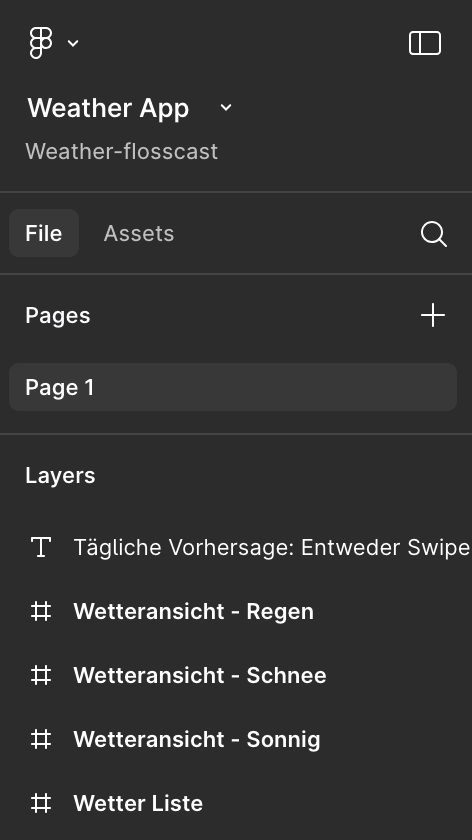
\includegraphics[width=0.35\textwidth]{figma_1.png}
\caption{Figma linke Ansicht}
\end{figure}

Auf der rechten Seite befinden sich die Einstellungen für die einzelnen Frames und deren Elemente, um diese zu bearbeiten und zu designen. Außerdem hat man die Option, die Größe des Prototyps jederzeit anzupassen und das Projekt in einer Vorschau vorzustellen bzw. zu teilen oder zu exportieren.

\begin{figure}[ht]
\centering
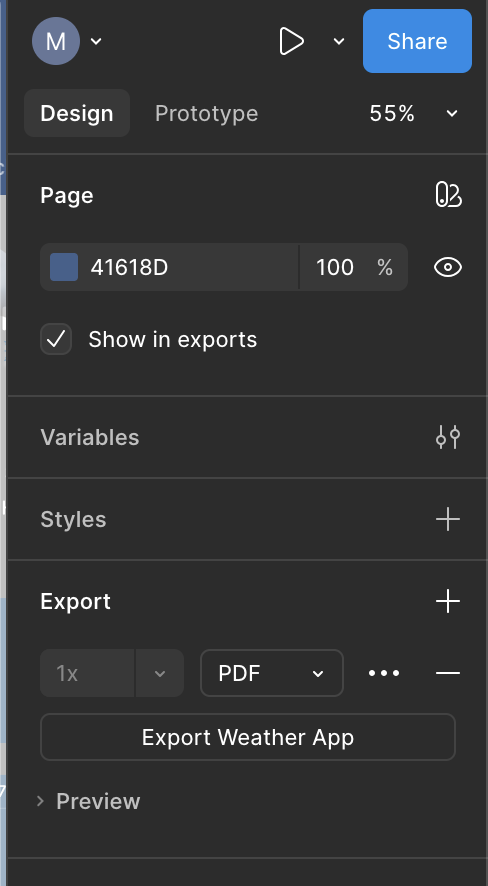
\includegraphics[width=0.35\textwidth]{figma_2.png}
\caption{Figma rechte Ansicht}
\end{figure}

\subsection{Planung}
Die Applikation sollte schlicht, übersichtlich, benutzerfreundlich
gestaltet sein und aus zwei Seiten bestehen. Die erste Seite hat die Funktion nach Städten bzw. Flughafen suchen zu können und diese mit den wichtigsten Informationen in der Liste darunter anzeigen zu lassen. Sobald man auf eine der Städte gedrückt hat, wird man auf die zweite Seite navigiert, die wiederum mehr Informationen bezüglich des Wetters von heute und die nächsten 7 Tage beinhaltet und bildlich darstellt, wie unter anderem der UV-Index oder die Niederschlagsmenge.

\subsection{Aufbau und Layout}
\subsubsection{Wetter Liste}
Der Hintergrund der Liste hat die Farbe schwarz und die Schriftfarbe ist in weiß. Beginnend von oben, ist links die Überschrift Wetter und rechts ein Dropdown-Menü, welches die Möglichkeit bietet, die Grad zahl in Celsius oder Fahrenheit darzustellen. Darunter gibt es eine Suchfunktion, um eine Stadt oder Flughafen suchen zu können. Daraufhin kann der gesuchte Ort gespeichert werden, um diesen in der Liste immer anzeigen lassen zu können. Die Liste besteht aus gespeicherten Orten, die die wichtigsten Informationen bezüglich des Wetters von heute darstellen. Sobald man auf einen der Orte drückt, expandiert sich das Fenster und eine vergrößerte Ansicht mit Informationen des Wetters, von heute und in den nächsten 7 Tage, wird angezeigt. 

\begin{figure}[ht]
\centering
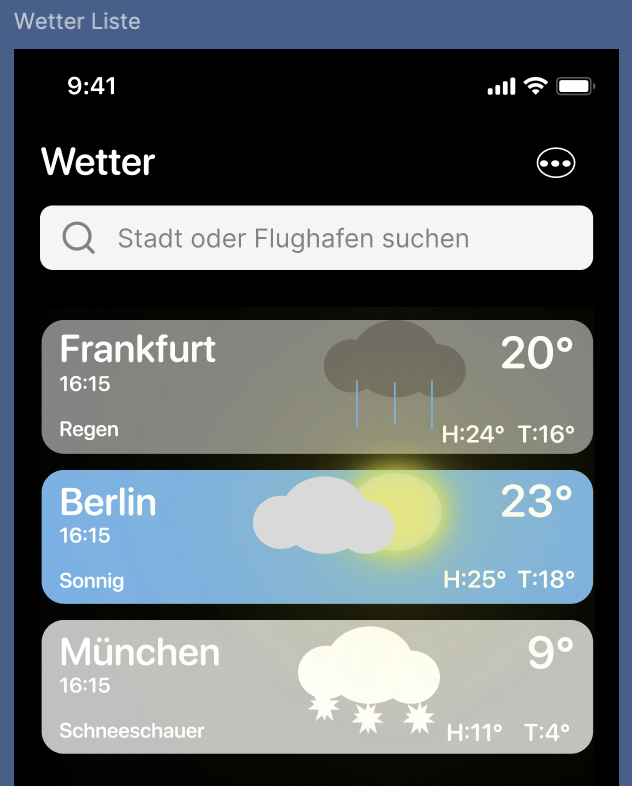
\includegraphics[width=0.35\textwidth]{wetterliste.png}
\caption{Wetter Liste}
\end{figure}

\subsubsection{Wetter Vorhersage}
Sobald man sich für ein Ort entschieden hat, entsteht eine vergrößerte Ansicht des Ortes mit passendem Hintergrund und Bild, welche abhängig von der Wetterlage ist. Es gibt drei Ansichten. Die erste stellt ein sonniges und die zweite ein regnerisches Wetter da. Die dritte stellt das Wetter beim Schneefall dar. Somit wird das derzeitige Wetterverhältnis bereits mit dem Bild ganz oben dargestellt mit zusätzlichen Informationen, wie der Ortsname, Ortsgrad, Ortswetter und die Höchst- bzw. Tiefst- Temperatur. Darunter befindet sich eine Box, die die Wettervorhersage stündlich für den heutigen Tag mit Bild und Grad ausgibt. Ähnlich ist es bei der zweiten Box, die wiederum das Wetter für die gesamte Woche mit Bild und Höchst- bzw. Tiefst- Temperatur darstellt. Für zusätzliche Informationen scrollt man nach unten und findet den UV-Index, die Windstärke bzw. Richtung und falls es Niederschlag gibt, die mm Anzahl.

\begin{figure}[htp]
\centering
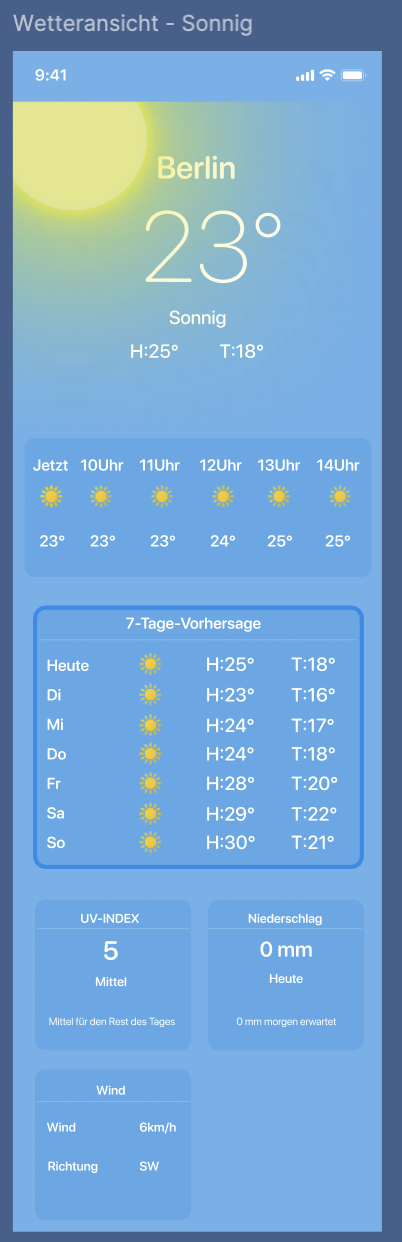
\includegraphics[width=0.3\textwidth]{wetter_sonnig.png}\hfill
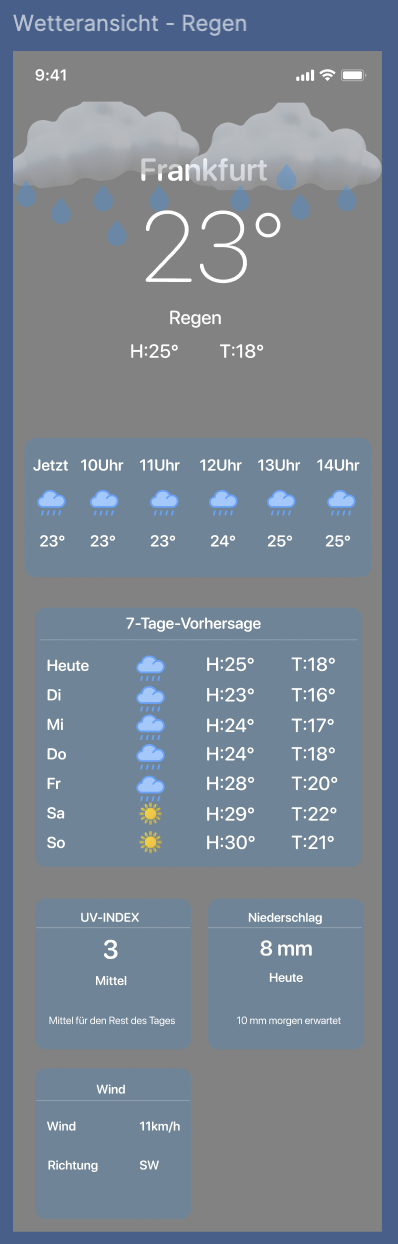
\includegraphics[width=0.3\textwidth]{wetter_regen.png}\hfill
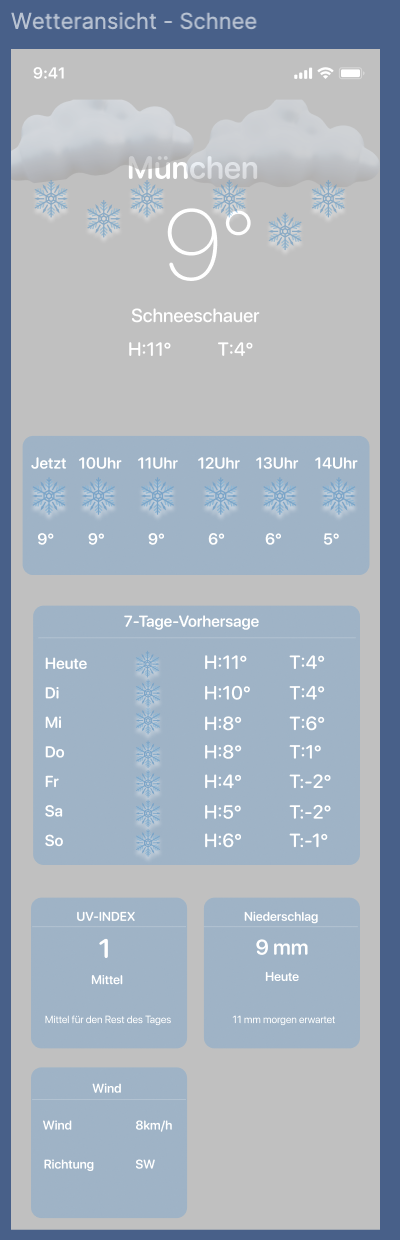
\includegraphics[width=0.3\textwidth]{wetter_schnee.png}
\caption{Wetter Vorhersagen}
\end{figure}

\section{Technische Dokumentation}
\subsection{Frontend \small{(Patryk Brychcy, Sascha Gavrilov)}}
\subsubsection{Einleitung}
Unsere Wetter-App besteht aus zwei Hauptbereichen: dem „SearchScreen“ zum Anlegen und Verwalten von Städten und dem „WeatherScreen“ zur Anzeige der aktuellen Wetterdaten und der Prognose für eine ausgewählte Stadt. Sobald die App gestartet wird, entscheidet MainActivity anhand der gespeicherten Städte, welcher Bildschirm zuerst angezeigt wird: entweder der Suchbildschirm, falls noch keine Städte hinterlegt sind, oder direkt die Wetteransicht für die zuletzt verwendeten Stadt.

\subsubsection{Architekturübersicht}
Die App ist nach dem klassischen Drei-Schichten-Prinzip aufgebaut.

In der Präsentationsschicht stellen Composable-Funktionen in SearchScreen.kt und WeatherScreen.kt die Benutzeroberfläche dar, reagieren auf Eingaben und visualisieren die aktuellen Wetterdaten.

Die Logik- und Aufbereitungsschicht in Utils.kt enthält alle Erweiterungsfunktionen, die die unbearbeiteten Forecast-Daten in gebrauchsfertige Teildaten umwandeln – etwa die momentane Temperatur, stündliche und tägliche Prognosewerte sowie die passenden Icons und Farben.

In der Datenhaltung schließlich übernimmt CityList.kt die Persistenz, indem es bis zu 30 Städte als Base64-kodiertes JSON in den SharedPreferences verwaltet.

So sind Darstellung, Geschäftslogik und Datenspeicherung sauber voneinander getrennt, was Wartung und Erweiterung der App erheblich erleichtert.

\subsubsection{MainActivity}
Die Navigation wird über einen NavHostController realisiert, der zwei Routen besitzt : „search“ für SearchScreen und „weather/{cityName}“ für WeatherScreen.

Beim Start liest MainActivity über CityList.getCities(context) die gespeicherten Städte ein. Bei einer leeren Liste navigiert die App automatisch zum Suchbildschirm und zeigt eine kurze Info „Keine Städte gespeichert“. Bei einer gefüllten Liste leitet die App direkt weiter zur Detailansicht der zuletzt genutzten Stadt (WeatherScreen(cityName)).

\subsubsection{SearchScreen}
SearchScreen ist der zentrale Bildschirm, auf dem Nutzer neue Städte suchen und ihre bereits gespeicherten Orte verwalten können. Oben befindet sich eine Suchleiste, in die man per Textfeld den Namen einer Stadt eingibt. Sobald man die Suche auslöst, leert die Liste zunächst alle vorherigen Suchergebnisse und zeigt dann passende Treffer in Form von NewCityCards an. Jede Karte repräsentiert eine Stadt mit Name, Bundesland und Land und lädt bei einem Tipp im Hintergrund über eine Coroutine den Forecast.

Gelingt die Abfrage, wird die Stadt in der Liste gespeichert (Duplikate anhand von Name, Bundesland und Land werden automatisch vermieden) und man springt direkt zur Detailansicht.

Gelingt die Abfrage nicht, erhält man lediglich einen kurzen Toast-Hinweis auf den Fehler.

Unterhalb der Suche zeigt CityListView alle bereits gespeicherten Städte als CityCards an. Jede CityCard enthält das aktuelle Wetter (Icon und Beschreibung), die momentane Temperatur, Minima und Maxima des Tages sowie einen Zeitstempel der letzten Aktualisierung.

Ein kurzer Tap auf eine CityCard öffnet die Detailseite, ein langer Druck ruft ein Bestätigungsdialog auf, mit dem man die Stadt aus der Liste entfernen kann. Beim ersten Laden der gespeicherten Städte oder beim Pull-to-Refresh blendet die App einen animierten Shimmer-Placeholder ein.

\subsubsection{WeatherScreen}

WeatherScreen zeigt alle relevanten Wetterinformationen für eine ausgewählte Stadt. Direkt beim Betreten lädt die App den Forecast über getForecastFromCacheOrDownload, entweder aus dem lokalen Cache oder frisch von der API. Über einen SwipeRefresh-Wrapper können Nutzer jederzeit nach unten wischen, um die Daten neu zu laden.

Im oberen Bereich, dem WeatherHeader, werden mithilfe der Funktion getWmoCodeAndIsNight() der WMO-Wettercode und der aktuelle Tag oder Nacht-Status ermittelt. Damit wählt die App automatisch die passende Lottie-Animation sowie die Hintergrundfarbe aus und zeigt in einer Spalte den Stadtnamen, die aktuelle Temperatur und einen kurzen Zustands-Text an.

Darunter folgt eine horizontale Stundenübersicht „HourlyForecastRow“, die in einer LazyRow 24 Stunden anzeigt. Jede HourlyItem-Karte besteht aus der Uhrzeit, Temperatur und dem entsprechenden Icon und liegt in einem leicht abgedunkelten Box-Hintergrund, um stets gut lesbar zu bleiben. Anschließend bietet der SevenDayForecastBlock eine Sieben-Tage-Prognose in Form von sieben Spalten: Jeder DailyItem zeigt den Tagesnamen („Heute“ oder Wochentag), die Regenwahrscheinlichkeit in Prozent, ein Icon sowie die Tageshöchst- und Tiefsttemperatur.

Ganz am Ende befindet sich die InfoBoxesSection mit vier Infoboxen: aktuelle Luftfeuchtigkeit, erwarteter Niederschlag für heute und morgen sowie Sonnenauf- und -untergangszeiten. Die Boxen liegen jeweils paarweise in zwei Zeilen, jede in einem verdunkeltem Hintergrund-Rahmen.

\subsubsection{Utils.kt}

In Utils.kt befinden sich Erweiterungsfunktionen, die die unbearbeiteten Forecast-Daten in übersichtliche Teildaten umwandeln. So liefert getCurrentTemperature() die Temperatur der aktuellen Stunde, getDailyMinTemp() und getDailyMaxTemp() ermitteln das Minimum und Maximum aus den 24 Stunden eines Tages. Die Funktion getHourlyData(offsetHours: Int) baut daraus ein HourlyData-Objekt mit Zeit, Temperatur, Zustand und Nacht-Flag, während getDailyData(day: Int) ein DailyData mit Label, Regenwahrscheinlichkeit, Min/Max und Icon-Code erstellt. Über Helper-Funktionen wie getLottieResForWmoCode, getIconForWmoCode, getConditionForWmoCode und colorForWmoCode wird jeweils basierend auf dem WMO-Code und dem Nacht-Status das richtige Icon, die passende Animation, der Beschreibungstext und die Hintergrundfarbe ausgewählt \cite{svgrepo}\cite{lottiefiles}. Eine Parallelisierungsfunktion loadForecastsForCities(context, cities) lädt Forecasts für mehrere Städte gleichzeitig und ermöglicht dadurch ein zügiges Nachladen im SearchScreen.

\subsubsection{CityList.kt}

CityList ist ein Singleton-Objekt, das die Persistenz aller Städte in den Android-SharedPreferences übernimmt. Es legt einen PREF-Datensatz („CityListPref“) an und speichert bis zu 30 Städte als Base64-kodiertes JSON. Mit getCities(context) liest es die aktuelle Liste aus, addCity(context, newCity) fügt eine Stadt vorne hinzu (und ersetzt dabei ein bestehendes Duplikat), removeCity(context, city) entfernt einen Eintrag, und clearCities(context) leert die gesamte Liste – nützlich zum Debuggen oder Reset. Intern sorgt eine einfache Duplikatprüfung dafür, dass Namen, Bundesland und Land übereinstimmen, bevor eine Stadt wirklich hinzugefügt wird, und bei einem Überschreiten der Listenlänge wird automatisch der älteste Eintrag entfernt.

\subsubsection{Zusammerfassung}

Dank der klaren Trennung zwischen den Composables für die Bildschirme, den Hilfsfunktionen in Utils.kt und der Persistenz in CityList.kt ist das Frontend genau strukturiert und leicht wartbar. Neue Features wie Favoriten oder erweiterte Details lassen sich durch zusätzliche Module ergänzen, ohne bestehende Teile anzupassen.

\subsection{Datenvorbereitung \small{(Benedikt Zundel)}}

Als Schnittstelle für die Wetterdaten haben wir uns für die \texttt{open-meteo} \cite{open-meteo} API entschieden, da diese alle Daten liefert die wir anzeigen wollten und über weitere Funktionalitäten wie geocoding verfügt. Um die Daten zu konsumieren, definierten wir zunächst ein Datenstruktur (vgl. listing \ref{lst:data-structure}) um die abgeholten Daten intern zu repräsentieren. Die Idee war es, dem frontend für den Konsum nur ein einzelnes Objekt zu übergeben, über das sinnvoll iteriert werden kann.

\begin{lstlisting}[label=lst:data-structure, caption=Forecast Datenstruktur]
data class Forecast(
    val timestamp: LocalDateTime,
    val days: List<DailyForecast>,
    val units: Units
)

data class DailyForecast(
    val date: LocalDate,
    val hourlyValues: List<Hourly>,
    val sunrise: LocalDateTime,
    val sunset: LocalDateTime
)

data class Hourly(
    val dateTime: LocalDateTime,
    val temperature: Double,
    val relativeHumidity: Int,
    val precipitationProbability: Int,
    val rain: Double,
    val showers: Double,
    val snowfall: Double,
    val weatherCode: Int
)

data class Units(
    val temperature: String,
    val humidity: String,
    val precipitationProbability: String,
    val rain: String,
    val showers: String,
    val snow: String,
)
\end{lstlisting}

Mittels Herangehensweisen aus der funktionalen Programmierung wie \texttt{map} lässt sich das von der API gelieferte JSON-Objekt mit wenig Aufwand, lesbar und modifizierbar in unsere Datenstruktur parsen (vgl. listing \ref{lst:parsing}).

\begin{lstlisting}[label=lst:parsing, caption=Auszug des Parsingprozesses]
val hourly: JsonObject = json["hourly"]!!.jsonObject
val hourlyTime =
    hourly.getOrThrow("time").jsonArray.map { LocalDateTime.parse(it.jsonPrimitive.content) }
val hourlyTemperature =
    hourly.getOrThrow("temperature_2m").jsonArray.map { it.jsonPrimitive.content.toDouble() }
...
val dailyForecasts: List<DailyForecast> = hourlyValues.groupBy { it.dateTime.date }
    .map { (date, measurements) -> DailyForecast(date
        , measurements
        , sunrise.first { it.date == date }.toInstant(TimeZone.UTC).toLocalDateTime(currentTimezone)
        , sunset.first { it.date == date }.toInstant(TimeZone.UTC).toLocalDateTime(currentTimezone)) }
\end{lstlisting}

Die Abfrageadresse ergibt sich aus Koordinaten die von Nutzer*innen als ausgewählte Stadt oder aktuellem Standort übergeben werden. Zur Realisierung der Städtewahl wird die selbe API unter dem geocoding Endpunkt angesprochen. Dieser liefert auf Basis eines (eventuell unvollständigem) Städtenamen eine Liste an bekannten Städten als Vorschläge, die dann in einem ähnlichen Prozess von JSON in eine von uns definierte Datenstruktur geparsed werden und dem frontend zum Anzeigen weitergegeben wird.

In dem gesamten Abfrageprozess wird hoher Wert auf die Richtigkeit der Daten und eine erfolgreiche Abwicklung der Anfragen gelegt. Viele der Schritte werden während der Verarbeitung der Daten gegen Erwartungswerte geprüft und unerwartete Situationen werden mittels Exceptions unmittelbar an das frontend kommuniziert. In Fehlersituation, sowie beim normalen Ablauf, wird eine Nachvollziehbarkeit des Prozesses mittels intensiven Loggings erreicht.

\subsection{Caching \small{(Benedikt Zundel)}}
Unnötige Abfragen werden zum Schutze des Verbrauchs der Nutzer*innen, sowie zur Entlastung der API unterbunden. Ein weiterer Nutzen ist die Verfügbarkeit der aktuellen Daten ohne Internetverbindung. Um das zu realisieren, implementieren wir ein dateibasiertes Caching-System. Die unterliegende Datei enthält die von der API abgeholten Wetterdaten nach unserer definierten Datenstruktur serialisiert in einem JSON-Objekt, welches die Daten via gekürztem Koordinatensatz indiziert. Durch das Kürzen der Koordinaten auf eine Nachkommastelle erreichen wir einen klein gehaltenen Datensatz der gecached wird, da nicht jede minimale Veränderung im Standort als neuer individuelle Standort angesehen wird. Der Standort wird durch die Kürzung auf circa $ 12 km \times 12 km $ Kacheln abgebildet, was, durch die kleine Fläche, zu keinem Genauigkeitsverlust führt.
Bei einem Aufruf der vom backend offengelegten Schnittstelle wird zunächst der Cache geladen und geprüft ob für die angefragten Koordinaten bereits ein Eintrag existiert. Sollte dies nicht der Fall sein, wird eine Abfrage auf die API gemacht und die Daten werden im Cache gespeichert. Wenn ein Eintrag gefunden wird, wird das Alter der Daten über ein Zeitstempel Feld geprüft. Ist ein Eintrag älter als eine Stunde, gilt dieser als veraltet und wird aktualisiert. Sonst wird der Eintrag aus dem Cache geladen und es geschieht keine Abfrage an die API.

\newpage

\bibliographystyle{plain}
\bibliography{refs}

\end{document}
